\documentclass{article}[18pt]
%\ProvidesPackage{format}
%Page setup
\usepackage[utf8]{inputenc}
\usepackage[margin=0.7in]{geometry}
\usepackage{parselines} 
\usepackage[english]{babel}
\usepackage{fancyhdr}
\usepackage{titlesec}
\hyphenpenalty=10000

\pagestyle{fancy}
\fancyhf{}
\rhead{Sam Robbins}
\rfoot{Page \thepage}

%Characters
\usepackage{amsmath}
\usepackage{amssymb}
\usepackage{gensymb}
\newcommand{\R}{\mathbb{R}}

%Diagrams
\usepackage{pgfplots}
\usepackage{graphicx}
\usepackage{tabularx}
\usepackage{relsize}
\pgfplotsset{width=10cm,compat=1.9}
\usepackage{float}

%Length Setting
\titlespacing\section{0pt}{14pt plus 4pt minus 2pt}{0pt plus 2pt minus 2pt}
\newlength\tindent
\setlength{\tindent}{\parindent}
\setlength{\parindent}{0pt}
\renewcommand{\indent}{\hspace*{\tindent}}

%Programming Font
\usepackage{courier}
\usepackage{listings}
\usepackage{pxfonts}

%Lists
\usepackage{enumerate}
\usepackage{enumitem}

% Networks Macro
\usepackage{tikz}


% Commands for files converted using pandoc
\providecommand{\tightlist}{%
	\setlength{\itemsep}{0pt}\setlength{\parskip}{0pt}}
\usepackage{hyperref}

% Get nice commands for floor and ceil
\usepackage{mathtools}
\DeclarePairedDelimiter{\ceil}{\lceil}{\rceil}
\DeclarePairedDelimiter{\floor}{\lfloor}{\rfloor}

% Allow itemize to go up to 20 levels deep (just change the number if you need more you madman)
\usepackage{enumitem}
\setlistdepth{20}
\renewlist{itemize}{itemize}{20}

% initially, use dots for all levels
\setlist[itemize]{label=$\cdot$}

% customize the first 3 levels
\setlist[itemize,1]{label=\textbullet}
\setlist[itemize,2]{label=--}
\setlist[itemize,3]{label=*}

% Definition and Important Stuff
% Important stuff
\usepackage[framemethod=TikZ]{mdframed}

\newcounter{theo}[section]\setcounter{theo}{0}
\renewcommand{\thetheo}{\arabic{section}.\arabic{theo}}
\newenvironment{important}[1][]{%
	\refstepcounter{theo}%
	\ifstrempty{#1}%
	{\mdfsetup{%
			frametitle={%
				\tikz[baseline=(current bounding box.east),outer sep=0pt]
				\node[anchor=east,rectangle,fill=red!50]
				{\strut Important};}}
	}%
	{\mdfsetup{%
			frametitle={%
				\tikz[baseline=(current bounding box.east),outer sep=0pt]
				\node[anchor=east,rectangle,fill=red!50]
				{\strut Important:~#1};}}%
	}%
	\mdfsetup{innertopmargin=10pt,linecolor=red!50,%
		linewidth=2pt,topline=true,%
		frametitleaboveskip=\dimexpr-\ht\strutbox\relax
	}
	\begin{mdframed}[]\relax%
		\centering
		}{\end{mdframed}}



\newcounter{lem}[section]\setcounter{lem}{0}
\renewcommand{\thelem}{\arabic{section}.\arabic{lem}}
\newenvironment{definition}[1][]{%
	\refstepcounter{lem}%
	\ifstrempty{#1}%
	{\mdfsetup{%
			frametitle={%
				\tikz[baseline=(current bounding box.east),outer sep=0pt]
				\node[anchor=east,rectangle,fill=blue!20]
				{\strut Definition};}}
	}%
	{\mdfsetup{%
			frametitle={%
				\tikz[baseline=(current bounding box.east),outer sep=0pt]
				\node[anchor=east,rectangle,fill=blue!20]
				{\strut Definition:~#1};}}%
	}%
	\mdfsetup{innertopmargin=10pt,linecolor=blue!20,%
		linewidth=2pt,topline=true,%
		frametitleaboveskip=\dimexpr-\ht\strutbox\relax
	}
	\begin{mdframed}[]\relax%
		\centering
		}{\end{mdframed}}
	
\newcounter{prob}[section]\setcounter{prob}{0}
\renewcommand{\theprob}{\arabic{section}.\arabic{lem}}
\newenvironment{problem}[1][]{%
	\refstepcounter{prob}%
	\ifstrempty{#1}%
	{\mdfsetup{%
			frametitle={%
				\tikz[baseline=(current bounding box.east),outer sep=0pt]
				\node[anchor=east,rectangle,fill=orange!20]
				{\strut Problem};}}
	}%
	{\mdfsetup{%
			frametitle={%
				\tikz[baseline=(current bounding box.east),outer sep=0pt]
				\node[anchor=east,rectangle,fill=orange!20]
				{\strut Problem:~#1};}}%
	}%
	\mdfsetup{innertopmargin=10pt,linecolor=orange!20,%
		linewidth=2pt,topline=true,%
		frametitleaboveskip=\dimexpr-\ht\strutbox\relax
	}
	\begin{mdframed}[]\relax%
	}{\end{mdframed}}
	
% Styling Pseudocode
\lstset{language=C,
	basicstyle=\ttfamily,
	keywordstyle=\bfseries,
	showstringspaces=false,
	morekeywords={if, else, then, print, end, for, do, while, Let},
	tabsize=4,
	mathescape=true,
	escapechar=£,
	numbers=left,
	stepnumber=1,
	frame=top,
	frame=bottom
}

\usepackage{caption}
\DeclareCaptionFormat{listing}{\rule{\dimexpr\textwidth+17pt\relax}{0.4pt}\par\vskip1pt#1#2#3}
\captionsetup[lstlisting]{format=listing,singlelinecheck=false, margin=0pt, font={sf},labelsep=space,labelfont=bf}


% Mathscr font
\usepackage{mathrsfs}

% Ensures there's a bit of the section before a new page
\preto{\subsection}{\Needspace{5\baselineskip}}
\preto{\section}{\Needspace{5\baselineskip}}
\lhead{AZ900}


\begin{document}
\begin{center}
\underline{\huge Azure Compute Options}
\end{center}
\section{Essential Azure compute concepts}
\begin{definition}[Virtual Machines]
	Software emulations of physical computers.
\end{definition}
\begin{definition}[Containers]
	A virtualization environment for running applications. Don't include an operating system for the apps running inside the container. Bundle the libraries and components needed to run the application and use the existing host OS running the container.
\end{definition}

\begin{definition}[Azure App Service]
	Platform as a service designed to host web oriented applications.
\end{definition}

\begin{definition}[Serverless Computing]
	Cloud hosted execution environment that runs your code but abstracts the underlying hosting environments.
\end{definition}
\section{Azure Virtual Machines}
VMs are an ideal choice when you need:
\begin{itemize}
	\item Total control over the OS
	\item The ability to run custom software
	\item To use custom hosting configurations
\end{itemize}
When to use virtual machines:
\begin{itemize}
	\item During testing and development
	\item When running applications in the cloud
	\item When extending your datacenter to the cloud
	\item During disaster recovery
\end{itemize}
\subsection{Scaling VMs}
\subsubsection{Availability set}
\begin{definition}[Availability set]
	A logical grouping of two or more VMs that help keep your application available during planned or unplanned maintenance.
\end{definition}
\begin{definition}[Planned maintenance event]
	When the underlying Azure fabric that hosts VMs is updated by Microsoft
\end{definition}
When the VM is part of an availability set, updates are sequenced so that not all the associated VMs are rebooted at the same time. They are put into different update domains
\begin{definition}[Update domains]
	Groups of VMs and underlying physical hardware that can be rebooted at the same time
\end{definition}
\begin{definition}[Unplanned maintenance]
	Hardware failure in the data centre, such as power outage or disk failure
\end{definition}
\begin{definition}[Fault domain]
	The group of virtual machines that all share common hardware that has failed.
\end{definition}
With an availability set you get:
\begin{itemize}
	\item Up to three fault domains that have a server rack with dedicated power and network resources
	\item Five logical update domains which then can be increased to 10
\end{itemize}
There is no cost for an availability set, just for the VMs in the set
\subsubsection{Virtual Machine Scale Sets}
Virtual machine scale sets let you create and manage a group of identical, load balanced VMs.\\
\\
This allows you to centrally manage, configure and update many VMs to provide highly available applications.
\subsubsection{Azure Batch}
Azure batch enables large scale job scheduling and compute management\\
\\
Batch:
\begin{itemize}
	\item Starts a pool of compute VMs for you
	\item Installs applications and staging data
	\item Runs jobs with as many tasks as you have
	\item Identifies failures
	\item Requeues work
	\item Scales down the pool as work completes
\end{itemize}

\section{Containers}
\subsection{Azure Container Instances}
PaaS to upload containers and execute them directly with automatic elastic scale
\subsection{Azure Kubernetes Service}
A complete orchestration service for containers with multiple architectures with multiple containers
\begin{definition}[Orchestration]
	The task of automating, managing and interacting with many containers
\end{definition}
\subsection{Microservice architecture}
Breaking solutions into smaller, independent pieces. This allows the separate components of the app to be maintained, scaled or updated independently.
\subsection{Migrating to containers}
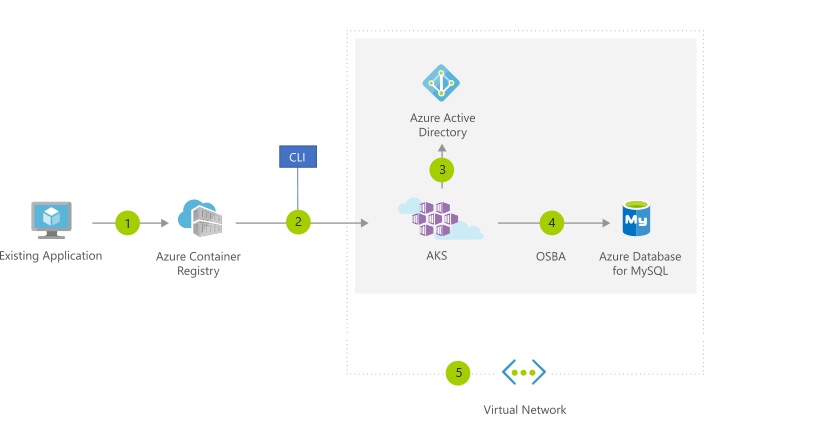
\includegraphics[width=15cm]{4-kub-migration}\\
The process is as follows:
\begin{enumerate}
	\item Convert the application to containers and publish to Azure Container Registry
	\item Deploy the containers to an AKS cluster
	\item Azure AD controls access to AKS resources
	\item You access Azure services
	\item Optionally, AKS is deployed with a virtual network
\end{enumerate}
\section{Azure App Service}
\subsection{Costs}
You pay for the compute resources your app uses. The app service plan determines how much hardware is devotes to the host. There's even a free tier for low traffic sites
\subsection{Types of app services}
\begin{itemize}
	\item Web apps - Host web apps
	\item API apps - Build REST-based Web APIs
	\item Web Jobs - Run a program or script in the same context as a web app. They can be scheduled or run by a trigger
	\item Mobile app back ends
	\begin{itemize}
		\item Store mobile app data in a cloud based SQL database
		\item Authenticate customers
		\item Send push notifications
		\item Execute custom back end logic
	\end{itemize}
\end{itemize}
\section{Serverless}
Serverless encompasses three ideas:
\begin{itemize}
	\item Abstraction of servers - Don't need to manage them
	\item Event-driven scale - Code runs when events come in
	\item Micro billing - Only pay for the time code runs
\end{itemize}
\subsection{Azure functions}
Azure functions are ideal for when you're only concerned about the code running your service. They commonly perform work in response to an event.\\
\\
Azure functions scale automatically based on demand.\\
\\
Azure functions can be either:
\begin{itemize}
	\item Stateless - Behave as if they've been restarted every time they respond to an event
	\item Stateful - A context is passed through the function to track prior activity
\end{itemize}
\subsection{Azure Logic Apps}
Logic apps execute workflows designed to automate business scenarios and built from predefined logic blocks.\\
\\
Every logic app workflow starts with a trigger. Azure Logic apps can be designed without code.
\subsection{Comparison}
{\renewcommand{\arraystretch}{2}
	\begin{tabularx}{\textwidth}{s b b}
		
		& \textbf{Functions} & \textbf{Logic apps}\\
		\hline
		Development& Code First & Designer First\\
		\hline
		Connectivity& Few built in bindings, write code for all else& large collection of connectors, write code for others\\
		\hline
		Actions& Each activity is an Azure function; write code for activity functions & Large collection of ready made functions\\
		\hline
		Monitoring& Azure application insights& Azure portal, Log Analytics\\
		\hline
		Management& REST API, Visual Studio& Azure portal, REST API, PowerShell, Visual Studio\\
		\hline
		Execution context& Locally and in cloud& Only in cloud
		
		
	\end{tabularx}
}
\end{document}
